\SourceLeaf{180}mals aus $q$ auf $MS$ das Perpendikel $qp'$, wo $p'$ zwischen $p$ und $M$
liegen wird. Sodann abermals aus $p'$ auf $NT$ das Perpendikel $p'q'$ u. s. w.
Diese Operationen lassen sich ohne Aufhören fortsetzen, und so werden von der
Linie $MS$ nach und nach die Stücke $Sp$, $pp'$ u. s. w. abgeschnitten, die jedes
eine angebliche Grösse haben, und deren Zahl unbegrenzt ist. Der Verfasser meint
nun, dass diess widersprechend sei, weil auf diese Weise nothwendig $MS$ zuletzt
erschöpft werden müsste. Es ist kaum begreiflich, wie er sich auf eine solche
Weise selbst täuschen konnte. Er macht sich sogar selbst den Einwurf, dass die
Summe der Stücke $Sp$, $pp'$ u. s. w., wenn diese Stücke immer kleiner und
kleiner werden, doch ungeachtet ihre Anzahl ohne Aufhören zunehme, nicht über
eine gewisse Grenze hinauswachsen könnte, und meint diesen Einwurf damit zu
heben, dass jene Stücke, auch wenn sie immer kleiner und kleiner werden, doch
  immer grösser bleiben, als eine \textls{angebliche Grösse}; nemlich jene Stücke
sind Katheten von rechtwinkligen Dreiecken, und folglich immer grösser als der
Unterschied zwischen Hypotenuse und der andern Kathete. Fast scheint es, dass
eine grammatische Zweideutigkeit den Verf. irre geleitet hat, nemlich der
  zwiefache Sinn des Artikels \textls{eine} angebliche Grösse. Der Schluss des
Verf. würde nur dann richtig sein, wenn sich zeigen liesse, dass die Stücke $Sp$,
  $pp'$ u. s. w. immer grösser bleiben als Eine \textls{bestimmte} angebliche
  Grösse, z. B. als der Unterschied zwischen der Hypotenuse $pT$ und der Kathete
$ST$. Aber das lässt sich nicht beweisen, sondern nur, dass jedes Stück immer
grösser bleibt, als eine angebliche Grösse, die aber selbst für jedes Stück eine
andere ist, nemlich $Sp$ grösser als der Unterschied zwischen $pT$ und $ST$,
ferner $pp'$ grösser als der Unterschied zwischen $qp'$ und $qp$ u. s. w.
Hiemit verschwindet nun aber die ganze Kraft des Beweises.

\begin{center}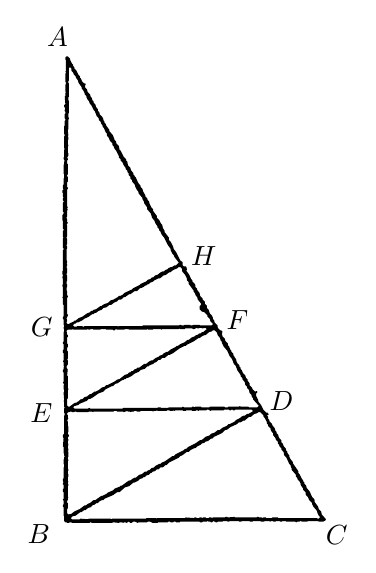
\begin{tikzpicture}[x=0.00764007cm,y=-0.00764007cm]
\fill[even odd rule] (98,82) -- (96,84) -- (96,87) -- (97,88) -- (97,106) -- (96,107) -- (97,109) -- (96,111) -- (96,124) -- (97,125) -- (97,128) -- (96,129) -- (96,140) -- (97,142) -- (96,143) -- (96,148) -- (95,149) -- (96,161) -- (94,163) -- (94,165) -- (96,169) -- (95,171) -- (95,173) -- (96,174) -- (96,177) -- (95,178) -- (95,185) -- (96,186) -- (96,188) -- (95,189) -- (95,197) -- (94,198) -- (94,211) -- (95,212) -- (95,214) -- (94,215) -- (94,234) -- (95,236) -- (94,237) -- (94,249) -- (93,250) -- (93,252) -- (95,256) -- (94,257) -- (94,261) -- (93,262) -- (93,277) -- (94,278) -- (94,284) -- (93,285) -- (93,295) -- (92,296) -- (92,301) -- (93,303) -- (91,305) -- (91,308) -- (92,309) -- (92,315) -- (93,316) -- (92,318) -- (92,321) -- (93,322) -- (93,324) -- (92,325) -- (92,340) -- (93,341) -- (93,343) -- (91,346) -- (91,354) -- (92,355) -- (92,368) -- (93,369) -- (93,371) -- (92,372) -- (92,382) -- (93,383) -- (92,385) -- (92,400) -- (93,401) -- (93,403) -- (92,404) -- (92,438) -- (91,439) -- (91,444) -- (92,445) -- (92,447) -- (91,448) -- (91,450) -- (92,451) -- (92,461) -- (91,462) -- (91,464) -- (92,465) -- (92,481) -- (91,483) -- (92,484) -- (92,494) -- (93,495) -- (93,514) -- (92,515) -- (92,518) -- (93,519) -- (93,528) -- (94,529) -- (94,531) -- (93,532) -- (93,534) -- (94,535) -- (94,539) -- (93,540) -- (93,556) -- (92,557) -- (92,559) -- (93,560) -- (93,569) -- (92,570) -- (92,574) -- (93,575) -- (93,587) -- (92,589) -- (93,590) -- (93,596) -- (94,598) -- (93,599) -- (93,602) -- (92,603) -- (92,606) -- (93,607) -- (93,622) -- (92,624) -- (94,627) -- (93,629) -- (93,635) -- (94,636) -- (94,639) -- (93,640) -- (94,653) -- (93,655) -- (94,656) -- (94,664) -- (95,665) -- (94,667) -- (94,674) -- (95,675) -- (95,678) -- (94,679) -- (94,709) -- (92,711) -- (92,715) -- (93,716) -- (92,730) -- (93,731) -- (93,741) -- (94,742) -- (94,745) -- (95,746) -- (94,748) -- (94,751) -- (93,752) -- (93,759) -- (94,760) -- (94,764) -- (93,765) -- (93,783) -- (92,784) -- (92,788) -- (93,789) -- (92,791) -- (92,793) -- (93,794) -- (93,800) -- (92,801) -- (92,805) -- (93,806) -- (93,817) -- (92,818) -- (93,820) -- (93,826) -- (92,827) -- (92,830) -- (93,831) -- (93,845) -- (94,846) -- (94,854) -- (96,856) -- (98,856) -- (99,857) -- (102,857) -- (103,856) -- (106,856) -- (107,857) -- (136,857) -- (137,856) -- (139,856) -- (140,857) -- (174,857) -- (175,856) -- (185,857) -- (186,856) -- (190,856) -- (192,857) -- (193,856) -- (196,856) -- (198,857) -- (201,855) -- (202,855) -- (204,857) -- (206,857) -- (209,855) -- (212,855) -- (216,857) -- (218,856) -- (232,856) -- (233,855) -- (237,855) -- (241,857) -- (249,857) -- (250,856) -- (266,856) -- (267,855) -- (270,855) -- (271,856) -- (275,856) -- (276,855) -- (279,855) -- (280,856) -- (286,856) -- (287,855) -- (319,855) -- (320,856) -- (323,856) -- (324,855) -- (331,855) -- (332,854) -- (334,855) -- (337,855) -- (338,856) -- (340,856) -- (342,854) -- (346,856) -- (348,856) -- (349,855) -- (357,855) -- (358,854) -- (365,854) -- (366,855) -- (368,855) -- (369,854) -- (384,854) -- (385,855) -- (388,855) -- (389,854) -- (402,854) -- (403,855) -- (407,855) -- (408,854) -- (420,854) -- (421,855) -- (426,855) -- (427,854) -- (435,854) -- (436,855) -- (438,854) -- (441,854) -- (442,855) -- (445,855) -- (446,854) -- (452,854) -- (453,855) -- (456,855) -- (457,854) -- (462,854) -- (463,855) -- (478,855) -- (480,856) -- (481,855) -- (485,855) -- (486,854) -- (488,854) -- (489,855) -- (498,855) -- (499,854) -- (516,854) -- (517,855) -- (524,855) -- (528,853) -- (529,851) -- (522,843) -- (521,838) -- (517,834) -- (516,830) -- (510,822) -- (510,819) -- (509,817) -- (506,814) -- (502,805) -- (497,799) -- (496,795) -- (493,792) -- (493,790) -- (491,788) -- (491,786) -- (489,784) -- (485,776) -- (483,774) -- (483,771) -- (474,758) -- (474,756) -- (470,751) -- (468,747) -- (468,745) -- (465,741) -- (465,739) -- (463,737) -- (462,733) -- (459,730) -- (457,725) -- (455,723) -- (455,720) -- (452,717) -- (450,713) -- (450,711) -- (447,708) -- (447,706) -- (445,704) -- (444,700) -- (440,695) -- (439,692) -- (435,688) -- (435,686) -- (433,684) -- (433,681) -- (431,679) -- (433,677) -- (434,677) -- (432,674) -- (430,674) -- (425,669) -- (421,661) -- (417,656) -- (416,652) -- (413,646) -- (413,642) -- (415,640) -- (415,639) -- (414,638) -- (411,639) -- (407,635) -- (406,632) -- (402,628) -- (402,625) -- (399,621) -- (399,619) -- (396,616) -- (395,612) -- (391,608) -- (389,603) -- (387,601) -- (387,599) -- (385,597) -- (385,595) -- (382,592) -- (380,588) -- (380,586) -- (375,578) -- (375,576) -- (372,573) -- (372,571) -- (370,569) -- (368,564) -- (366,562) -- (366,559) -- (362,555) -- (361,551) -- (357,547) -- (357,545) -- (356,544) -- (357,539) -- (355,537) -- (353,537) -- (350,534) -- (349,532) -- (349,529) -- (344,524) -- (343,520) -- (341,518) -- (341,516) -- (339,512) -- (336,509) -- (334,503) -- (331,500) -- (331,496) -- (328,493) -- (328,490) -- (324,486) -- (324,484) -- (320,480) -- (319,475) -- (315,470) -- (315,468) -- (312,465) -- (312,462) -- (311,460) -- (307,456) -- (307,454) -- (305,452) -- (302,445) -- (297,438) -- (298,436) -- (297,432) -- (296,431) -- (293,431) -- (291,429) -- (291,424) -- (287,421) -- (280,407) -- (276,402) -- (275,398) -- (271,390) -- (268,387) -- (268,383) -- (261,374) -- (261,372) -- (258,367) -- (257,362) -- (255,360) -- (252,354) -- (248,350) -- (248,347) -- (242,339) -- (242,336) -- (239,333) -- (236,327) -- (235,323) -- (233,321) -- (232,318) -- (229,315) -- (229,313) -- (225,306) -- (224,302) -- (221,299) -- (221,297) -- (217,292) -- (213,283) -- (211,281) -- (211,280) -- (209,278) -- (209,276) -- (205,271) -- (204,267) -- (200,263) -- (199,257) -- (197,255) -- (197,253) -- (193,249) -- (188,239) -- (186,237) -- (185,231) -- (181,227) -- (180,223) -- (178,221) -- (175,213) -- (169,206) -- (169,204) -- (164,197) -- (163,194) -- (161,192) -- (161,190) -- (159,188) -- (159,186) -- (157,182) -- (153,178) -- (153,176) -- (150,172) -- (150,170) -- (147,166) -- (146,162) -- (143,159) -- (143,157) -- (141,155) -- (140,151) -- (138,149) -- (137,145) -- (133,141) -- (132,137) -- (129,134) -- (129,130) -- (130,128) -- (129,127) -- (127,127) -- (124,124) -- (122,119) -- (120,117) -- (120,115) -- (118,113) -- (114,105) -- (111,102) -- (111,100) -- (109,98) -- (109,96) -- (107,94) -- (104,88) -- (104,86) -- (100,82) -- cycle
(519,847) -- (519,848) -- (517,850) -- (515,850) -- (514,849) -- (450,849) -- (449,848) -- (440,848) -- (439,849) -- (430,849) -- (429,848) -- (425,848) -- (423,849) -- (422,848) -- (418,848) -- (417,847) -- (415,847) -- (414,848) -- (378,848) -- (377,847) -- (366,848) -- (365,847) -- (362,847) -- (361,848) -- (341,848) -- (340,849) -- (338,848) -- (335,848) -- (334,849) -- (330,849) -- (329,848) -- (325,848) -- (324,849) -- (322,848) -- (319,848) -- (318,849) -- (314,849) -- (313,848) -- (311,848) -- (310,849) -- (296,848) -- (295,849) -- (249,849) -- (248,850) -- (246,849) -- (231,849) -- (230,850) -- (174,850) -- (173,851) -- (171,850) -- (135,850) -- (134,851) -- (121,850) -- (120,851) -- (107,851) -- (105,849) -- (108,846) -- (113,845) -- (121,839) -- (123,839) -- (127,836) -- (129,836) -- (134,832) -- (138,831) -- (142,827) -- (144,827) -- (148,824) -- (150,824) -- (153,821) -- (157,819) -- (159,819) -- (161,817) -- (175,811) -- (182,806) -- (186,806) -- (195,798) -- (202,796) -- (209,790) -- (211,790) -- (217,787) -- (220,784) -- (224,783) -- (226,781) -- (228,781) -- (231,778) -- (235,777) -- (238,774) -- (239,774) -- (241,772) -- (245,771) -- (248,768) -- (251,768) -- (254,765) -- (257,765) -- (259,764) -- (262,761) -- (264,761) -- (268,757) -- (284,749) -- (287,746) -- (290,745) -- (298,739) -- (301,739) -- (304,736) -- (310,733) -- (312,733) -- (315,730) -- (321,727) -- (323,725) -- (327,724) -- (329,722) -- (333,721) -- (338,717) -- (340,717) -- (343,714) -- (356,708) -- (361,703) -- (365,702) -- (370,698) -- (381,693) -- (384,690) -- (387,690) -- (392,687) -- (394,687) -- (401,681) -- (404,681) -- (410,676) -- (414,675) -- (417,673) -- (420,673) -- (425,678) -- (425,680) -- (428,684) -- (431,690) -- (431,692) -- (433,694) -- (433,696) -- (437,700) -- (437,702) -- (439,706) -- (441,708) -- (441,711) -- (445,716) -- (446,719) -- (449,722) -- (449,725) -- (451,727) -- (452,730) -- (455,733) -- (455,735) -- (459,740) -- (459,743) -- (460,745) -- (463,748) -- (468,759) -- (470,761) -- (471,765) -- (472,766) -- (472,769) -- (479,777) -- (479,780) -- (481,782) -- (482,785) -- (485,788) -- (487,792) -- (487,794) -- (491,800) -- (491,802) -- (495,806) -- (495,809) -- (496,811) -- (499,814) -- (501,819) -- (506,824) -- (506,826) -- (508,830) -- (514,837) -- (515,841) -- (517,845) -- cycle
(407,670) -- (407,672) -- (400,676) -- (398,676) -- (394,679) -- (392,679) -- (388,681) -- (386,683) -- (380,686) -- (377,689) -- (369,693) -- (367,693) -- (364,696) -- (357,699) -- (352,703) -- (349,703) -- (344,707) -- (338,709) -- (335,712) -- (329,714) -- (323,719) -- (319,720) -- (312,725) -- (300,731) -- (297,734) -- (295,734) -- (293,736) -- (279,743) -- (276,746) -- (274,746) -- (261,755) -- (256,757) -- (254,759) -- (252,759) -- (246,762) -- (243,765) -- (239,766) -- (236,769) -- (233,770) -- (231,772) -- (228,772) -- (223,776) -- (219,777) -- (213,782) -- (211,782) -- (207,784) -- (205,786) -- (201,787) -- (190,795) -- (188,795) -- (186,797) -- (178,800) -- (175,803) -- (166,807) -- (164,809) -- (158,812) -- (156,812) -- (146,819) -- (143,819) -- (137,824) -- (134,825) -- (130,828) -- (128,828) -- (120,834) -- (111,838) -- (106,842) -- (101,843) -- (99,841) -- (99,834) -- (100,833) -- (100,824) -- (99,823) -- (99,820) -- (100,819) -- (100,816) -- (101,815) -- (100,813) -- (100,796) -- (101,795) -- (101,793) -- (100,792) -- (100,790) -- (101,789) -- (100,787) -- (100,781) -- (101,780) -- (101,776) -- (100,775) -- (100,771) -- (101,770) -- (101,768) -- (100,767) -- (100,755) -- (101,754) -- (101,752) -- (100,751) -- (100,748) -- (101,747) -- (101,739) -- (100,738) -- (101,736) -- (101,734) -- (100,733) -- (100,729) -- (101,728) -- (101,726) -- (100,725) -- (100,721) -- (101,720) -- (101,718) -- (100,717) -- (100,715) -- (102,713) -- (102,711) -- (100,709) -- (100,707) -- (101,706) -- (101,697) -- (100,696) -- (100,689) -- (99,687) -- (101,683) -- (100,682) -- (100,678) -- (99,677) -- (99,675) -- (101,673) -- (103,673) -- (104,672) -- (106,672) -- (107,673) -- (111,673) -- (112,672) -- (114,672) -- (115,673) -- (134,673) -- (135,672) -- (140,672) -- (142,673) -- (143,672) -- (176,672) -- (177,671) -- (181,671) -- (182,672) -- (192,672) -- (193,673) -- (199,671) -- (200,672) -- (203,672) -- (205,673) -- (206,672) -- (210,672) -- (211,671) -- (214,671) -- (215,672) -- (220,672) -- (221,671) -- (240,671) -- (242,672) -- (243,671) -- (247,671) -- (248,670) -- (250,671) -- (264,671) -- (265,670) -- (269,670) -- (270,671) -- (274,671) -- (275,670) -- (277,671) -- (279,670) -- (291,670) -- (292,671) -- (296,671) -- (297,670) -- (306,670) -- (307,671) -- (312,671) -- (313,670) -- (315,670) -- (317,671) -- (318,670) -- (330,670) -- (331,669) -- (334,669) -- (337,671) -- (339,670) -- (359,670) -- (360,669) -- (368,669) -- (369,670) -- (371,670) -- (372,669) -- (374,669) -- (375,670) -- (377,670) -- (378,669) -- (406,669) -- cycle
(417,662) -- (417,663) -- (415,665) -- (401,665) -- (400,664) -- (387,664) -- (386,663) -- (384,664) -- (367,664) -- (366,665) -- (361,665) -- (360,664) -- (336,664) -- (335,665) -- (322,665) -- (321,664) -- (312,664) -- (310,665) -- (309,664) -- (307,664) -- (306,665) -- (293,665) -- (291,664) -- (290,665) -- (268,665) -- (267,666) -- (255,666) -- (254,665) -- (250,665) -- (249,666) -- (192,666) -- (191,667) -- (137,667) -- (136,666) -- (134,667) -- (111,667) -- (109,665) -- (111,663) -- (118,661) -- (120,659) -- (132,654) -- (135,651) -- (137,651) -- (141,649) -- (151,642) -- (159,639) -- (163,635) -- (173,630) -- (175,630) -- (179,626) -- (183,625) -- (190,620) -- (192,620) -- (194,618) -- (196,618) -- (198,616) -- (200,616) -- (206,613) -- (211,609) -- (218,606) -- (221,603) -- (228,601) -- (232,597) -- (234,597) -- (236,595) -- (242,593) -- (244,591) -- (247,590) -- (251,586) -- (254,586) -- (257,583) -- (261,583) -- (267,578) -- (269,578) -- (275,575) -- (286,567) -- (294,563) -- (296,563) -- (298,561) -- (310,555) -- (317,550) -- (319,550) -- (323,547) -- (327,545) -- (329,545) -- (335,540) -- (339,539) -- (341,537) -- (344,537) -- (348,541) -- (349,545) -- (353,550) -- (354,554) -- (356,556) -- (356,558) -- (359,564) -- (365,571) -- (369,580) -- (373,585) -- (376,593) -- (379,596) -- (382,604) -- (387,611) -- (387,613) -- (390,616) -- (390,618) -- (394,623) -- (395,628) -- (398,631) -- (398,633) -- (401,636) -- (402,641) -- (405,644) -- (406,648) -- (408,650) -- (408,652) -- cycle
(331,535) -- (325,540) -- (323,540) -- (321,542) -- (319,542) -- (315,545) -- (313,545) -- (311,547) -- (306,549) -- (301,553) -- (299,553) -- (294,557) -- (287,560) -- (283,563) -- (281,563) -- (279,565) -- (271,569) -- (266,573) -- (264,573) -- (260,575) -- (257,578) -- (253,579) -- (251,581) -- (246,583) -- (241,587) -- (239,587) -- (235,589) -- (230,593) -- (227,593) -- (219,599) -- (216,599) -- (214,601) -- (211,602) -- (208,605) -- (206,605) -- (204,607) -- (202,607) -- (199,610) -- (195,611) -- (186,618) -- (182,619) -- (178,622) -- (166,628) -- (164,628) -- (161,631) -- (157,632) -- (152,636) -- (146,639) -- (144,639) -- (142,641) -- (141,641) -- (139,643) -- (137,643) -- (132,647) -- (128,648) -- (125,651) -- (121,652) -- (118,655) -- (117,655) -- (115,657) -- (111,658) -- (103,664) -- (101,664) -- (99,662) -- (99,651) -- (100,650) -- (100,637) -- (101,636) -- (101,634) -- (100,633) -- (100,613) -- (99,612) -- (100,602) -- (98,599) -- (98,597) -- (100,594) -- (100,587) -- (99,586) -- (100,584) -- (100,572) -- (99,571) -- (99,566) -- (100,565) -- (100,560) -- (99,559) -- (99,549) -- (100,548) -- (100,545) -- (99,544) -- (98,538) -- (100,536) -- (107,536) -- (108,535) -- (110,536) -- (132,536) -- (133,535) -- (135,536) -- (137,536) -- (138,535) -- (142,535) -- (143,536) -- (154,536) -- (155,535) -- (163,535) -- (164,536) -- (175,536) -- (176,537) -- (178,537) -- (180,535) -- (182,536) -- (194,536) -- (195,535) -- (201,535) -- (202,536) -- (231,536) -- (232,535) -- (234,536) -- (241,536) -- (242,535) -- (254,535) -- (256,536) -- (257,535) -- (284,535) -- (285,534) -- (287,535) -- (294,535) -- (295,534) -- (307,534) -- (308,535) -- (310,535) -- (314,533) -- (316,534) -- (318,534) -- (319,533) -- (322,533) -- (323,534) -- (329,533) -- cycle
(341,526) -- (341,527) -- (339,529) -- (320,529) -- (319,528) -- (308,528) -- (307,529) -- (304,529) -- (303,528) -- (294,528) -- (293,529) -- (289,529) -- (288,528) -- (286,528) -- (285,529) -- (225,529) -- (224,530) -- (185,530) -- (184,531) -- (182,530) -- (128,530) -- (127,531) -- (125,531) -- (124,530) -- (116,530) -- (115,531) -- (111,531) -- (109,529) -- (109,528) -- (111,526) -- (113,526) -- (115,524) -- (117,524) -- (125,520) -- (127,518) -- (134,515) -- (141,510) -- (143,510) -- (145,508) -- (147,508) -- (151,505) -- (156,503) -- (159,500) -- (164,499) -- (169,495) -- (172,495) -- (177,491) -- (182,489) -- (185,486) -- (188,486) -- (190,485) -- (193,482) -- (195,482) -- (202,477) -- (204,477) -- (211,472) -- (215,472) -- (220,467) -- (222,467) -- (226,465) -- (228,463) -- (230,463) -- (232,461) -- (235,460) -- (237,458) -- (242,456) -- (244,454) -- (250,451) -- (253,451) -- (259,446) -- (263,445) -- (268,441) -- (270,441) -- (275,437) -- (282,434) -- (284,432) -- (287,432) -- (289,434) -- (290,436) -- (290,439) -- (295,445) -- (298,451) -- (298,454) -- (301,457) -- (301,460) -- (309,471) -- (309,473) -- (311,475) -- (313,480) -- (315,482) -- (316,486) -- (321,492) -- (321,495) -- (319,497) -- (319,502) -- (323,506) -- (327,507) -- (332,512) -- (332,514) -- (336,518) -- (337,522) -- cycle
(104,100) -- (106,102) -- (106,105) -- (107,107) -- (109,109) -- (110,112) -- (113,115) -- (114,118) -- (117,122) -- (118,126) -- (123,133) -- (123,135) -- (126,139) -- (128,143) -- (128,145) -- (131,148) -- (131,150) -- (133,154) -- (135,156) -- (137,161) -- (139,163) -- (143,171) -- (145,173) -- (148,181) -- (151,184) -- (152,188) -- (155,191) -- (155,193) -- (158,197) -- (158,199) -- (160,201) -- (163,208) -- (165,210) -- (165,213) -- (166,215) -- (168,217) -- (170,222) -- (174,226) -- (174,229) -- (176,231) -- (178,236) -- (180,238) -- (185,248) -- (185,250) -- (188,253) -- (188,255) -- (191,258) -- (193,263) -- (196,267) -- (196,269) -- (199,272) -- (199,274) -- (201,276) -- (201,279) -- (204,282) -- (204,285) -- (207,288) -- (207,290) -- (212,296) -- (212,298) -- (215,304) -- (217,306) -- (218,310) -- (224,317) -- (224,319) -- (227,324) -- (227,326) -- (232,333) -- (232,336) -- (238,343) -- (240,350) -- (244,355) -- (246,360) -- (249,364) -- (249,366) -- (252,369) -- (252,371) -- (254,373) -- (256,378) -- (260,383) -- (266,395) -- (271,402) -- (271,404) -- (274,410) -- (276,412) -- (277,415) -- (284,424) -- (284,425) -- (280,429) -- (278,429) -- (273,432) -- (271,432) -- (267,434) -- (265,436) -- (262,437) -- (260,439) -- (258,439) -- (254,441) -- (249,445) -- (245,446) -- (242,449) -- (240,449) -- (237,452) -- (233,453) -- (230,456) -- (221,460) -- (219,462) -- (209,467) -- (207,469) -- (194,475) -- (191,478) -- (187,480) -- (185,480) -- (183,482) -- (176,486) -- (172,487) -- (166,492) -- (162,493) -- (158,495) -- (156,497) -- (154,497) -- (147,502) -- (143,503) -- (141,505) -- (139,505) -- (137,507) -- (132,509) -- (125,514) -- (118,517) -- (113,521) -- (111,521) -- (109,523) -- (104,525) -- (102,527) -- (100,527) -- (98,525) -- (98,523) -- (99,522) -- (98,517) -- (100,513) -- (100,511) -- (99,510) -- (99,483) -- (100,482) -- (100,480) -- (99,479) -- (99,472) -- (98,471) -- (98,466) -- (99,465) -- (99,461) -- (98,460) -- (98,456) -- (99,455) -- (99,446) -- (98,445) -- (98,443) -- (99,442) -- (99,434) -- (98,433) -- (98,431) -- (99,430) -- (99,427) -- (98,426) -- (99,424) -- (99,422) -- (98,421) -- (98,402) -- (99,401) -- (99,398) -- (98,397) -- (98,395) -- (99,394) -- (99,385) -- (98,384) -- (98,382) -- (99,381) -- (99,363) -- (98,361) -- (100,359) -- (100,358) -- (99,357) -- (99,352) -- (98,351) -- (98,349) -- (99,348) -- (99,338) -- (100,337) -- (99,335) -- (100,333) -- (99,331) -- (99,303) -- (100,302) -- (100,300) -- (99,299) -- (99,291) -- (100,290) -- (100,282) -- (99,281) -- (99,279) -- (100,278) -- (100,261) -- (99,260) -- (99,255) -- (100,254) -- (100,252) -- (99,250) -- (101,247) -- (101,243) -- (100,242) -- (100,232) -- (101,231) -- (101,229) -- (100,228) -- (100,221) -- (101,220) -- (101,216) -- (100,215) -- (101,213) -- (100,204) -- (101,203) -- (101,187) -- (102,186) -- (102,184) -- (101,183) -- (101,177) -- (102,176) -- (102,156) -- (101,155) -- (101,150) -- (102,149) -- (102,127) -- (101,126) -- (101,123) -- (102,122) -- (102,101) -- cycle;
\node[inner sep=0pt] at (83,50) {$A$};
\node[inner sep=0pt] at (326,413) {$H$};
\node[inner sep=0pt] at (57,532) {$G$};
\node[inner sep=0pt] at (382,520) {$F$};
\node[inner sep=0pt] at (56,674) {$E$};
\node[inner sep=0pt] at (455,655) {$D$};
\node[inner sep=0pt] at (52,875) {$B$};
\node[inner sep=0pt] at (547,878) {$C$};
\end{tikzpicture}
\end{center}

Auf dieselbe Art, wie er seinen Beweis führen zu können geglaubt hat, könnte er
auch beweisen, dass in einem ebenen Dreiecke $ABC$, worin $B$ ein rechter Winkel
ist, $C$ nicht spitz sein könne; er brauchte nur aus $B$ ein Perpendikel $BD$ auf
die Hypotenuse $AC$ zu fällen, dann wieder das Perpendikel $DE$ auf $AB$ und so
ohne Aufhören die Perpendikel $EF$, $FG$, $GH$ u. s. w. wechselsweise auf $AC$
und $AB$.] Die Stücke $CD$, $DF$, $FH$ u. s. w.
